\documentclass{article}
\usepackage{a4wide}
\usepackage{float}
\usepackage{graphicx, latexsym, longtable}
\usepackage{epsfig, color, psfrag}
\usepackage{amsmath, amsfonts, amssymb}
\usepackage{multirow}
\usepackage{fancyvrb}
\usepackage{subfig}
\captionsetup[subfigure]{labelformat=empty}
\usepackage[ 
pdfauthor={Xu Xiang},
pdftitle={Weighted Finite State Transducer Components Construction},
pagebackref=false,
colorlinks=false,
linkcolor=red,
]{hyperref}

\begin{document}
\bibliographystyle{plain}

\begin{titlepage}
\hrule

\vspace{0.2in}
\begin{center}
{\bf Weighted Finite State Transducer Components Construction\\}
\bigskip
Xu Xiang\\
\smallskip
\date
\bigskip

E-mail: {\tt chinoiserie811@gmail.com}\\

\bigskip

\bigskip

\end{center}

\vspace{2cm}

\hrule

\bigskip

\abstract 
The weighted finite state transducer (WFST) framework provides a general representation for components of speech recognition systems, including acoustic model, context-dependency model, pronounciation model and statistical language model. We investigate several approaches and schemes of constructing WFST components used in IDIAP's Juicer WFST decoder and Josef Novak's Transducersaurus WFST tool sets. We illustrate the model to WFST construction progress to address some more general problems, and attempt to achieve some reasonable results.
\endabstract
\bigskip
\hrule

\end{titlepage}

\tableofcontents \listoffigures \listoftables

\newpage
\setcounter{page}{1}
\section{Introduction}
\label{sec:intro}

WFST~\cite{mohri2008speech, mohri2009weighted} has been widely used in the area of automatic speech recognition (ASR). In ASR system designs, WFST is used to represent models at different stages such as acoustic model (denoted by H), context-dependency model (denoted by C), pronunciation model (denoted by L), statistical language model (denoted by G), etc. There are several rules and conventions to construct WFST from these models, however, it is sometimes tricky to tune the construction progress to make the resulting WFST more efficient and robust.

This technical report examines both Juicer and Transducersaurus, and compares their WFST construction approaches.

This technical report is arranged as follows. 
Section~\ref{sec:grmmod} describes the statistical language model to WFST construction and discusses about normalisation and auxiliary symbols.
Section~\ref{sec:lexmod} describes the pronunciation model to WFST construction and covers the topic of optimization.
Section~\ref{sec:cdmod} illustrates a simple example of context-dependency model to WFST construction.
Conclusions are drawn in section~\ref{sec:conclusion}.


\section{Statistical language model to WFST}
\label{sec:grmmod}

\subsection{$n-$gram Language Model Format}
\label{subsubsec:ngramformat}

The word level grammar G, often a stochastic $n-$gram, can be represented by WFST compactly~\cite{allauzen2003generalized}. The basic idea of constructing WFST from $n-$gram, can be described by the following rules (\href{http://openfst.cs.nyu.edu/twiki/bin/view/GRM/NGramModelFormat}{OpenGrm project NGram Model Format} by Michael Riley \textit{et al}.). \vspace{5mm}

An n-gram is a sequence of $k$ symbols: $w_1\cdots{}w_k$. Let $\mathbb{N}$ be the set of n-grams in the model.

\begin{itemize}
\item
  There is a \textit{unigram} state in every model, representing the empty string.
\item
  Every proper prefix of every n-gram in $\mathbb{N}$ has an associated state in the model.
\item
  The state associated with an n-gram $w_1\cdots{}w_k$ has a backoff transition (labeled with $\langle epsilon\rangle$) to the state associated with its suffix $w_2\cdots{}w_k$.
\item
  An n-gram $w_1\cdots{}w_k$ is represented as a transition, labeled with $w_k$, from the state associated with its prefix $w_1\cdots{}w_{k-1}$ to a destination state defined as follows:
  \begin{itemize}
  \item
    If $w_1\cdots{}w_k$ is a proper prefix of an $n-$gram in the model, then the destination of the transition is the state associated with $w_1\cdots{}w_k$.
  \item
    Otherwise, the destination of the transition is the state associated with the suffix $w_2\cdots{}w_k$.
  \end{itemize}
\item
  Start and end of the sequence are not represented via transitions in the automaton or symbols in the symbol table. Rather
  \begin{itemize}
  \item
    The start state of the automaton encodes the ``start of sequence'' $n-$gram prefix (commonly denoted $\langle s\rangle$).
  \item
    The end of the sequence (often denoted $\langle /s\rangle$) is included in the model through state final weights, i.e., for a state associated with an $n-$gram prefix $w_1\cdots{}w_k$, the final weight of that state represents the weight of the $n-$gram $w_1\cdots{}w_k \langle /s\rangle$.
  \end{itemize}
\end{itemize}

\newpage
There is a small but complete bigram language model in ARPA format. Notice that the probabilities are base 10 logarithms.

\begin{Verbatim}[frame=none, framesep=5mm]
\data\
ngram 1=4
ngram 2=6

\1-grams:
-99 <s> -0.39794
-0.69897 </s>
-0.39794 foo -0.60206
-0.39794 bar -0.60206

\2-grams:
-0.251812 <s> foo
-0.4436975 <s> bar
-0.6478175 foo foo
-0.139662 foo bar
-0.3716111 bar </s>
-0.3233064 bar foo

\end\
\end{Verbatim}

\begin{figure}[H]
  \centering
  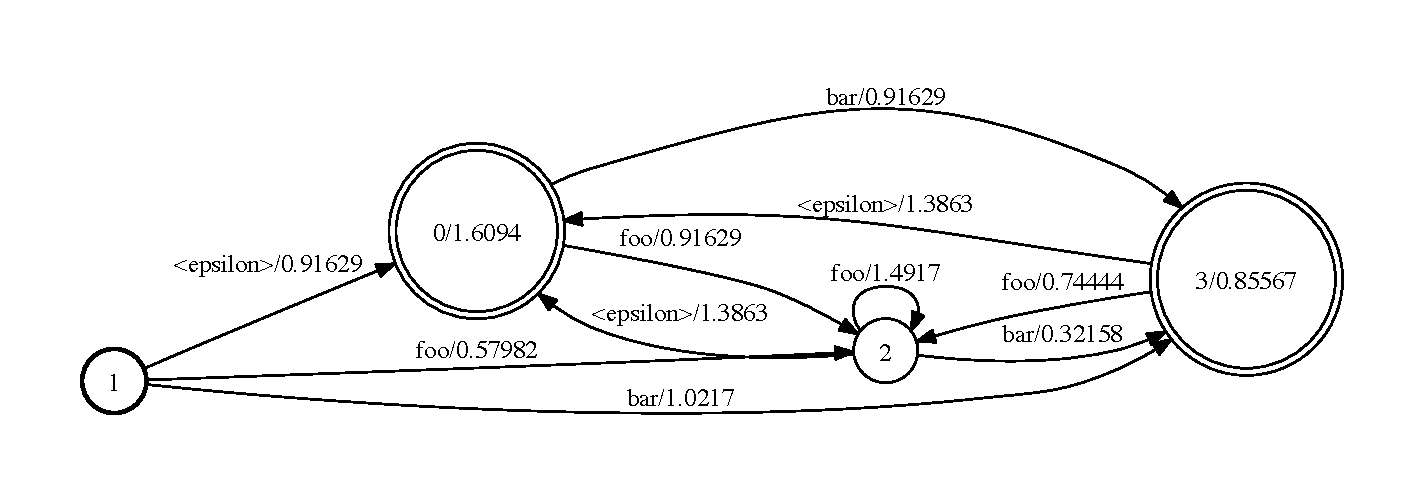
\includegraphics[width=\textwidth]{./figures/opengrm_2g.pdf}
  \caption{A bigram language model constructed by OpenGrm (ngrammake)}
\end{figure}

The model format used by Juicer and Transducersaurus is almost the same as OpenGrm NGram Format, except for

\begin{itemize}
\item
  There is a additional ``start'' state which only has one transition (labeled with $\langle s\rangle$) to the state associated with the ``start of sequence'' $n-$gram prefix (commonly denoted $\langle s\rangle$)
\item
  There is a additional ``end'' state (commonly denoted $\langle /s\rangle$). The end of the sequence (denoted $\langle /s\rangle$) is included in the model through a transition (labeled with $\langle /s\rangle$) to the ``end'' state. The weight of the transition represents the weight of the $n-$gram $w_1\cdots{}w_k \langle /s\rangle$. Thus, all successful paths are ended at this unique ``end'' state.
\end{itemize}

Figure~\ref{gramgen} depicts the G WFST constrcuted by gramgen.

\begin{figure}[H]
  \centering
  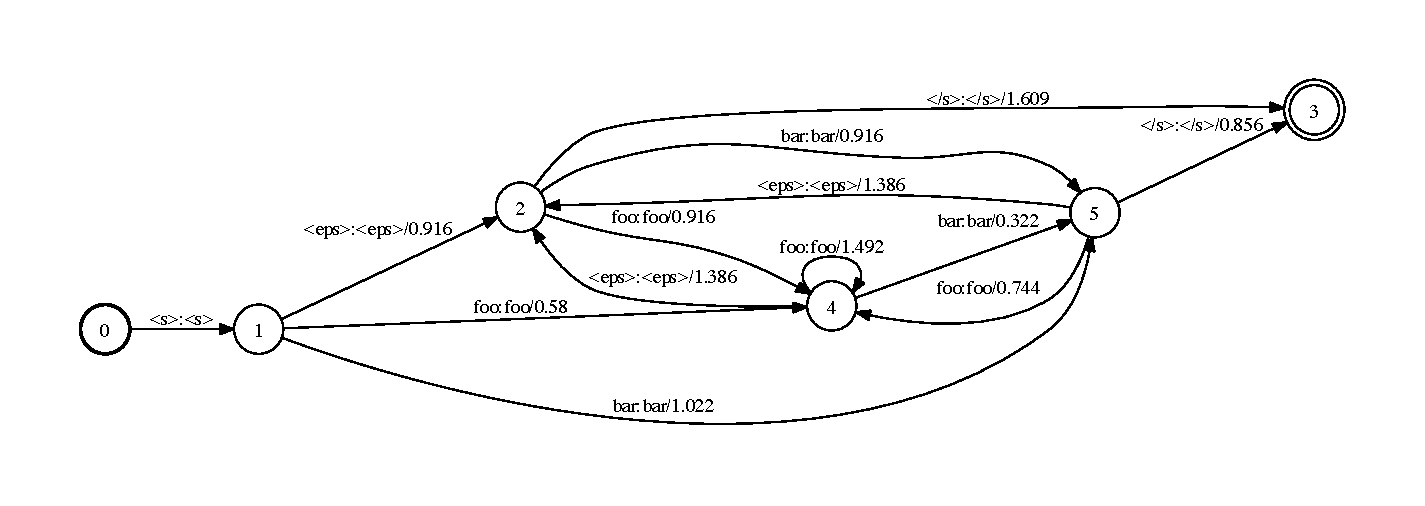
\includegraphics[width=\textwidth]{./figures/juicer_2g.pdf}
  \caption{A bigram language model constructed by Juicer (gramgen)}
  \label{gramgen}
\end{figure}

\subsection{Auxiliary Labels on Backoff $\epsilon-$Transitions}
\label{subsubsec:grmaux}
In the presence of backoff $\epsilon-$transitions, G may have several paths for a given word sequence. In this case, we can disambiguate the model by replacing the input $\epsilon-$label on backoff transitions with the auxiliary label (usually denoted by $\phi-$label). Respectively, We need to apply auxiliary symbols to L properly. By introducing auxiliary labels to G and L, we can ensure the composite WFST of L$^{*}$ (Kleene closure) and G is deterministic.

If we compose L$^{*}$ and G with matching filter without auxiliary symbols, we may get a non-deterministic and larger result as depicted in Figure~\ref{non-deterministic-LG}. An easier solution is using sequencing filter instead. Figure~\ref{deterministic-LG} shows the deterministic resulting WFST using sequencing filter, which can be optimized further.

Figure~\ref{lg_aux} shows that the same resulting WFST of composing L$^{*}$ and G by applying auxiliary symbols.

To reduce the size and facilitate the optimization of the composite WFST, it is encouraged to implement auxiliary symbols on L and G.

\begin{figure}[H]
  \centering
  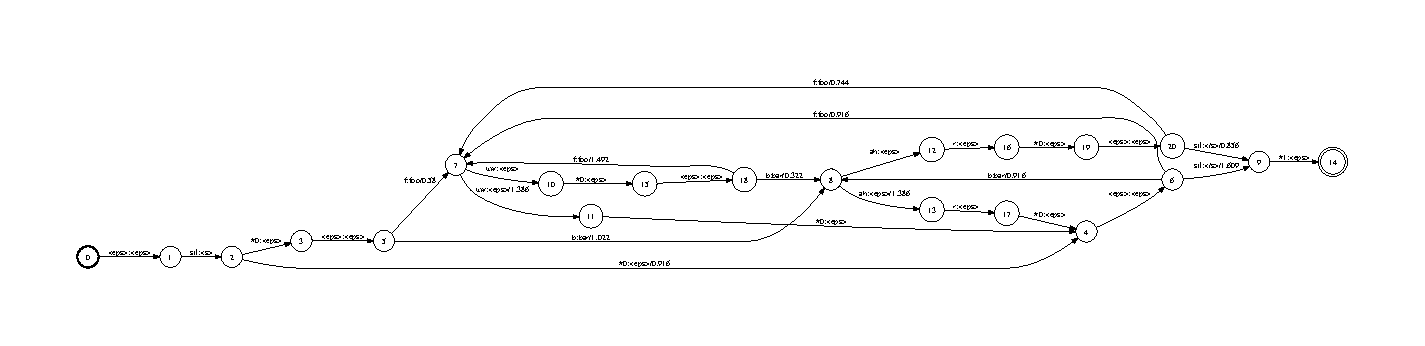
\includegraphics[width=\textwidth]{./figures/match_without_phi.pdf}
  \caption{Compose L$^{*}$ and G using matching filter, without auxiliary labels}
  \label{non-deterministic-LG}
\end{figure}

\begin{figure}[H]
  \centering
  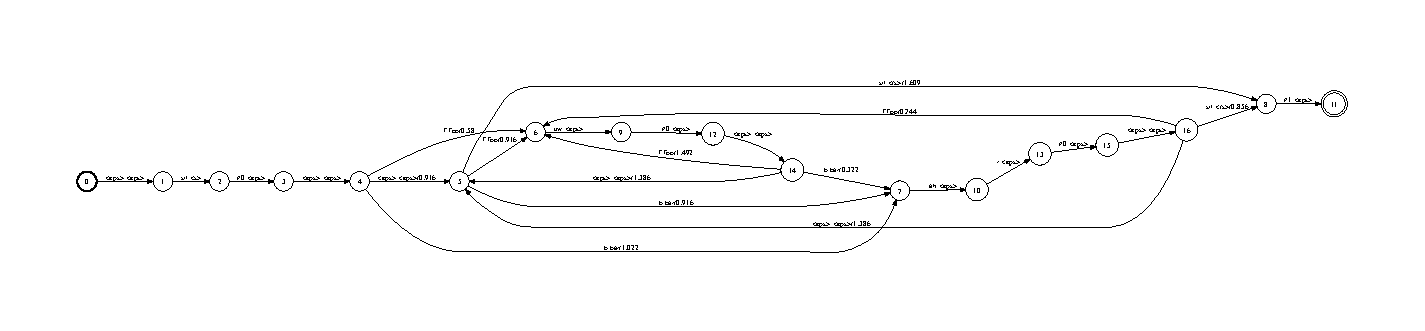
\includegraphics[width=\textwidth]{./figures/seq_without_phi.pdf}
  \caption{Compose L$^{*}$ and G using sequencing filter, without auxiliary labels}
  \label{deterministic-LG}
\end{figure}

\begin{figure}[H]
  \centering
  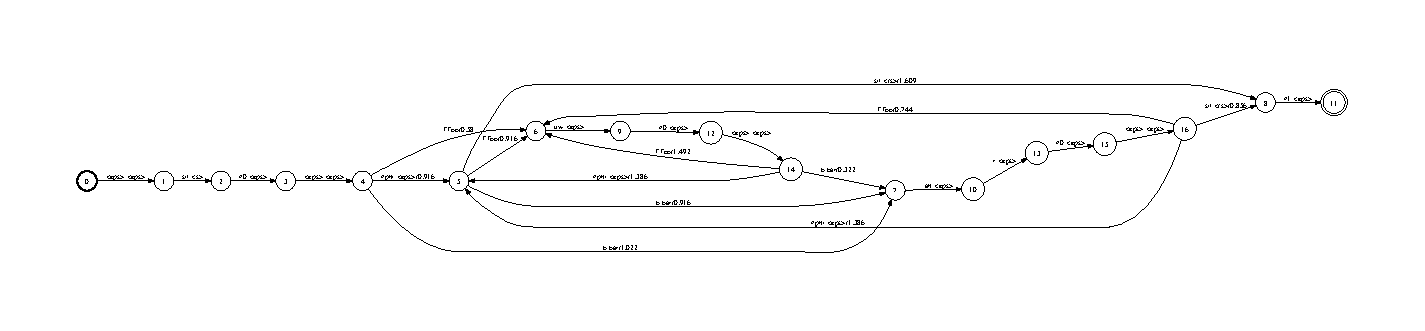
\includegraphics[width=\textwidth]{./figures/lg_with_phi.pdf}
  \caption{Compose L$^{*}$ and G, with auxiliary labels}
  \label{lg_aux}
\end{figure}


\subsection{$n-$gram Language Model Normalisation}
\label{subsubsec:grmnorm}
In practice, $n-$gram language models are trained on very large corpus. An unmodified language model is usually too large for practical use, so there are several pruning techniques to produce a smaller language model. However, some probability (seen $n-$grams) may be ``disgarded'' after pruning. To keep the stochasticity, the backoff weights need to be re-estimated. 

For example, the equation for Katz's backoff model~\cite{katz1987estimation} is
$$
\hat{P}(w_{i}|w_{i-n+1}\cdots{}w_{i-1}) = \left\{
\begin{aligned}
d_{w_{i-n+1}\cdots{}w_{i}}\frac{C(w_{i-n+1}\cdots{}w_{i})}{C(w_{i-n+1}\cdots{}w_{i-1})} \mbox{ if } C(w_{i-n+1}\cdots{}w_{i}) > k,\\
\alpha_{w_{i-n+1}\cdots{}w_{i-1}}\hat{P}(w_{i}|w_{i-n+2}\cdots{}w_{i-1}) \mbox{ otherwise.}\\
\end{aligned}
\right.
$$
where,

$C(x)$ is the number of times $x$ appears in training.

$w_{i}$ is the $i$th word in the given context.

$d$ is typically the amount of discounting found by Good-Turing estimation.

Thus the backoff weight $\alpha$ is computed as
$$
\alpha_{w_{i-n+1}\cdots{}w_{i-1}} = \frac{1-\sum\limits_{\{w_{i}:C(w_{i-n+1}\cdots{}w_{i})>k\}}d_{w_{i-n+1}\cdots{}w_{i}}\frac{C(w_{i-n+1}\cdots{}w_{i})}{C(w_{i-n+1}\cdots{}w_{i-1})}}{\sum\limits_{\{w_{i}:C(w_{i-n+1}\cdots{}w_{i})\leq{k}\}}\hat{P}(w_{i}|w_{i-n+2}\cdots{}w_{i-1})}
$$

\section{Pronunciation model to WFST}
\label{sec:lexmod}

\subsection{Basic Representation}
\label{subsubsec:lexrep}

From the simple dictionary below, we can construct an L WFST. Figure~\ref{lex} depicts the L WFST.

\begin{Verbatim}[frame=none, framesep=5mm]
<s> sil
</s> sil
bar b ah r
foo f uw
\end{Verbatim}

\begin{figure}[H]
  \centering
  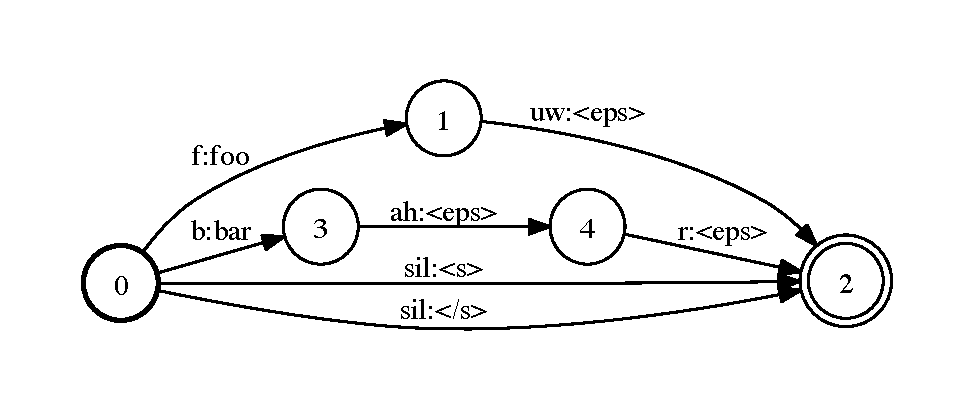
\includegraphics[width=0.6\textwidth]{./figures/lex.pdf}
  \caption{A simple L WFST}
  \label{lex}
\end{figure}

\subsection{Auxiliary Labels}
\label{lexaux}
In general, L is not determinizable in the presence of homophony. To make L determinizable, we need to introduce auxiliary symbols to L. For example\\

\texttt{r eh d \#0} read

\texttt{r eh d \#1} red \\

Let P denotes the maximum degree of the homophony. Then we add P different auxiliary phones.

We need to add a $\phi-$loop at the start state of L. This $\phi-$loop is both to match the $\phi-$labels in G WFST, and to propagate them to the composite WFST of L$^{*}$ and G. 
We also need to add other auxiliary labels (one of \#0, \#1, ... \#P-1) to the end of the phonetic transcription of each word to distinguish homophones. In practice we use the transformed L$^{*}$ to compose.

Figure~\ref{lexstar} depicts the transformed L$^{*}$ WFST.

\begin{figure}[H]
  \centering
  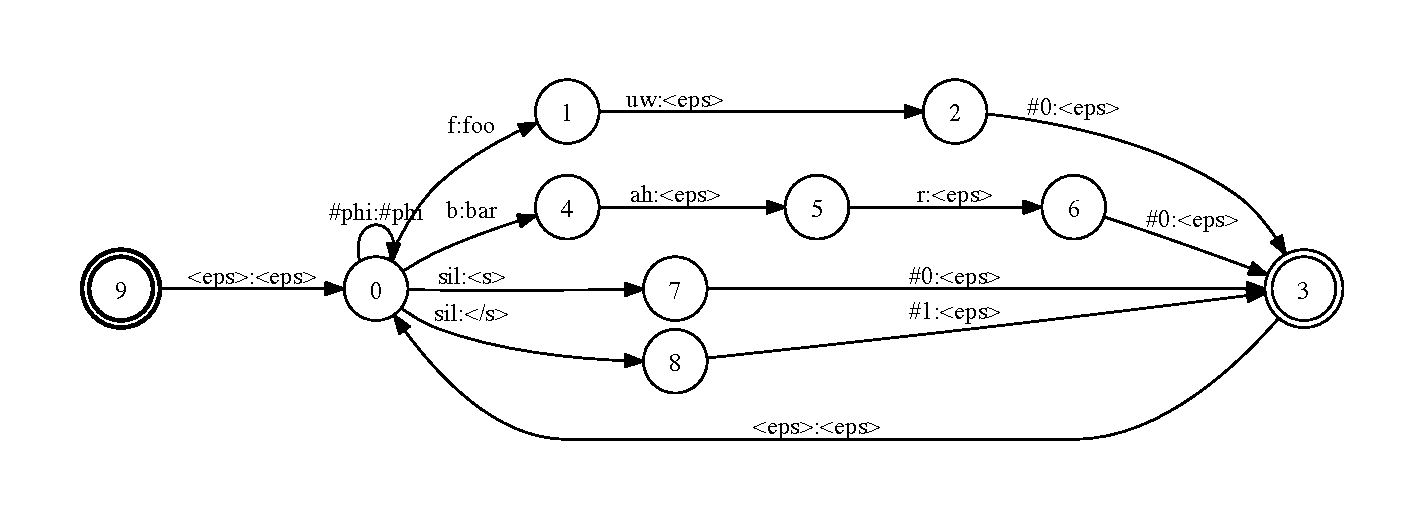
\includegraphics[width=\textwidth]{./figures/lex_star.pdf}
  \caption{A transformed L$^{*}$ WFST}
  \label{lexstar}
\end{figure}

\subsection{Optimization Issues}
\label{lexopt}

We performed experiments on a 4 core Intel Core i3-3220 based machine running at 3.30GHz with 3MB cache and 8GBs of main system memory running GNU/Linux. We evaluated the composing progress using the standard WSJ 5k close NVP bigram language model and the WSJ 5k non-verbalized vocabulary.

To compose L$^{*}$ and G in a standard way, it's preferable not to optimize the L$^{*}$ WFST, since it's optimized to leave the output label in place. Table~\ref{tbl:stdLG} shows the differences of two configurations that optimizes $\tilde{\text{L}}$ or not. The $\circ$ denotes to the standard composition.

\begin{table}[H]
\begin{center}
  \begin{tabular}{| c | c | c | c |}
  \hline
  Composition Configuration & Time & Memory Usage & WFST Size \\ \hline
  $\tilde{\text{L}}\circ\tilde{\text{G}}$ & 0.542s & 47MB & 20MB \\ \hline
  det($\tilde{\text{L}})\circ\tilde{\text{G}}$ & 31.262s & 3.7GB & 891MB \\ \hline
  \end{tabular}
  \caption{Standard composition of $\tilde{\text{L}}$ and $\tilde{\text{G}}$}
  \label{tbl:stdLG}
\end{center}
\end{table}

To compose CL WFST and G WFST with static lookahead approach, C and L$^{*}$ are composed first to produce CL WFST. In this case, it's preferable to determinize L$^{*}$ first. Table~\ref{tbl:lkhCLG} shows the differences of two configurations that optimizes $\tilde{\text{L}}$ or not. The $\circ$ denotes to the standard composition, and the $.$ denotes to the lookahead composition.

\begin{table}[H]
\begin{center}
  \begin{tabular}{| c | c | c | c |}
  \hline
  Composition Configuration & Time & Memory Usage & WFST Size  \\ \hline
  $\tilde{\text{C}}\circ\tilde{\text{L}}$ & 1.601s & 121MB & 68MB \\ \hline
  $(\tilde{\text{C}}\circ\tilde{\text{L}}).\tilde{\text{G}}$ & 4.163s & 315MB & 109MB \\ \hline
  $\tilde{\text{C}}\circ{}det(\tilde{\text{L}})$ & 0.074s & -MB & 1.4MB \\ \hline
  $(\tilde{\text{C}}\circ{}det(\tilde{\text{L}})).\tilde{\text{G}}$ & 3.321s & 183MB & 38MB \\ \hline
  \end{tabular}
  \caption{Static lookahead composition of $\tilde{\text{C}}\tilde{\text{L}}$ and $\tilde{\text{G}}$}
  \label{tbl:lkhCLG}
\end{center}
\end{table}

\section{Context-dependency model to WFST}
\label{sec:cdmod}

\subsection{Sub-word Units}
\label{sec:subword}
The context dependency model maps sequences of context dependency phones (the sub-word units presented in a GMM based acoustic model) to sequences of monophones (the sub-word units used in a pronunciation model).

There are two variants of context-dependency models using different strategies to cope with \textit{word boundary} information. One is word-internal model, and the other is cross-word model. The example below shows the differences of these two methods. 

For simplicity, we will focus on the cross-word context dependency model in subsequent discussions. \vspace{5mm}

\textbf{Word-internal} context dependency:

Word boundaries represent a distinct context.
\begin{Verbatim}[frame=leftline, framesep=5mm]
speech task =
/sil s+p s-p+iy p-iy+ch iy-ch
t+ae t-ae+s ae-s+k s-k sil/
\end{Verbatim}

\textbf{Cross-word} context dependency:

Word boundaries are ignored or used as additional context information.
\begin{Verbatim}[frame=leftline, framesep=5mm]
speech task = 
/sil sil-s+p s-p+iy p-iy+ch iy-ch+t
ch-t+ae t-ae+s ae-s+k s-k+sil sil/
\end{Verbatim}

\subsection{Basic Representation} 
\label{cdrep}

Basically, the C WFST is constructed by the rules~\cite{dixonintroduction} stated in Table~\ref{tbl:cdrules}.
 
\begin{table}[H]
\begin{center}
  \begin{tabular}{| c | c | c | c | c |}
  \hline
  Type & Source & Destination & Input Symbol & Output Symbol \\ \hline
  l-c+r & l,c & c,r & l-c+r & r \\ \hline
  c+r & -,c & c,r & c+r & r \\ \hline
  l-c & l,c & c,-(Final) & l-c & - \\ \hline
  c & -,-(Start) & -,c & - & c \\ \hline
  c & -,c & c,-(Final) & c & - \\ \hline
  \end{tabular}
  \caption{Context dependency model to WFST construction rules}
  \label{tbl:cdrules}
\end{center}
\end{table}

Figure~\ref{c_prototype} shows a prototype C WFST, the context independent phones are $x$ and $y$ only.

\begin{figure}[H]
  \centering
  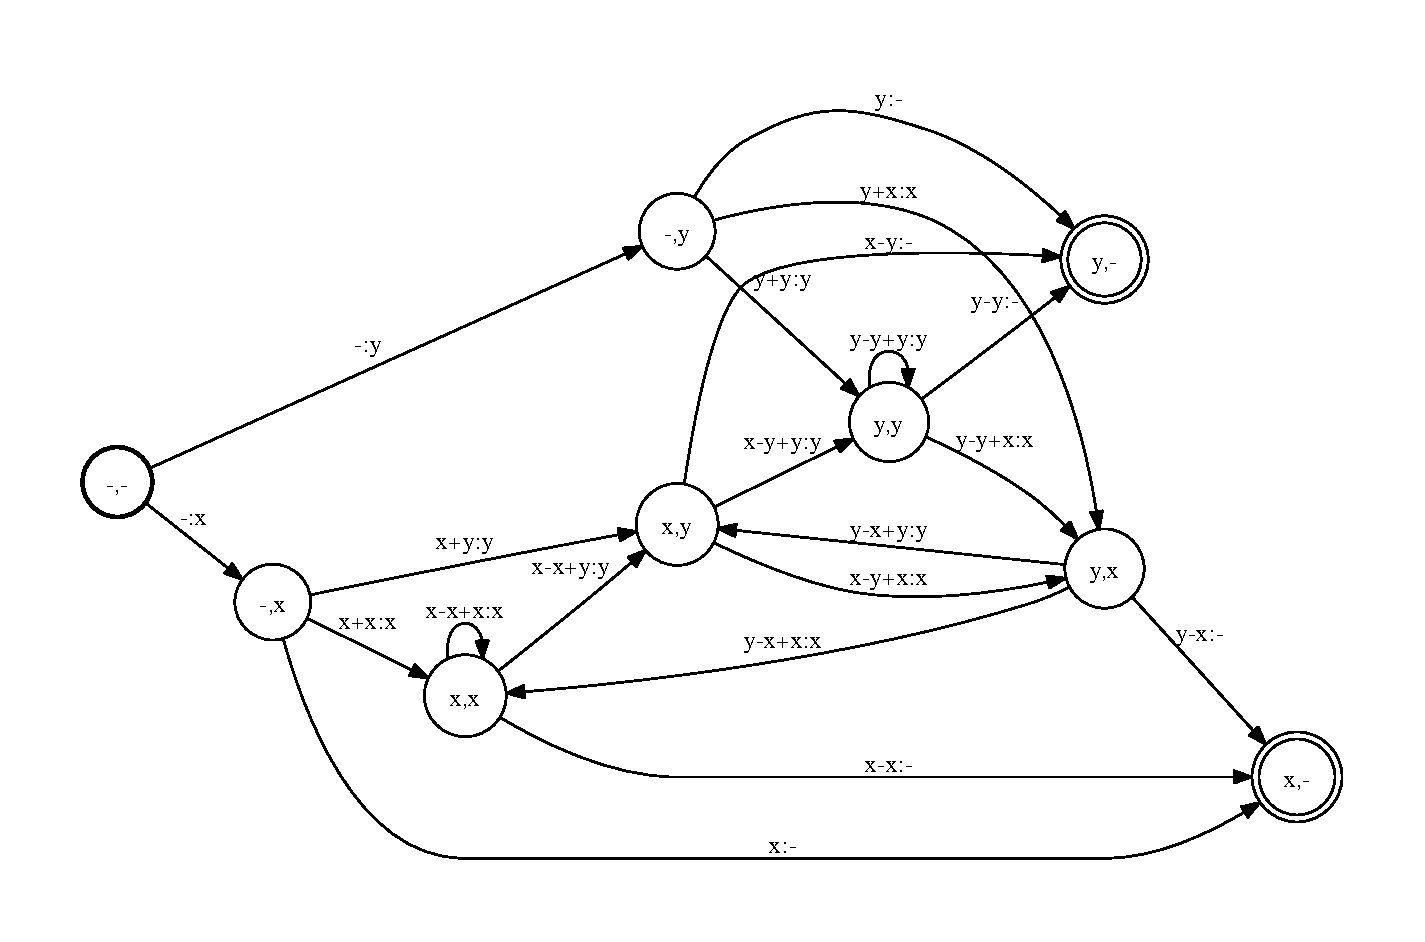
\includegraphics[width=0.7\textwidth]{./figures/c_prototype.pdf}
  \caption{A prototype C WFST}
  \label{c_prototype}
\end{figure}

There is a very small emparical C WFST constructed by Juicer (cdgen) depicted in Figure~\ref{c_no_sp_aux}. Notice that we assume that all logical triphones are physical triphones. We use only one silence model ``sil'' and the auxiliary symbols are not illustrated. All triphones in tiedlist are in set $\{sil\}\cup\{f,uw,sil\}\times\{f,uw\}\times\{f,uw,sil\}$.

\begin{figure}[H]
  \centering
  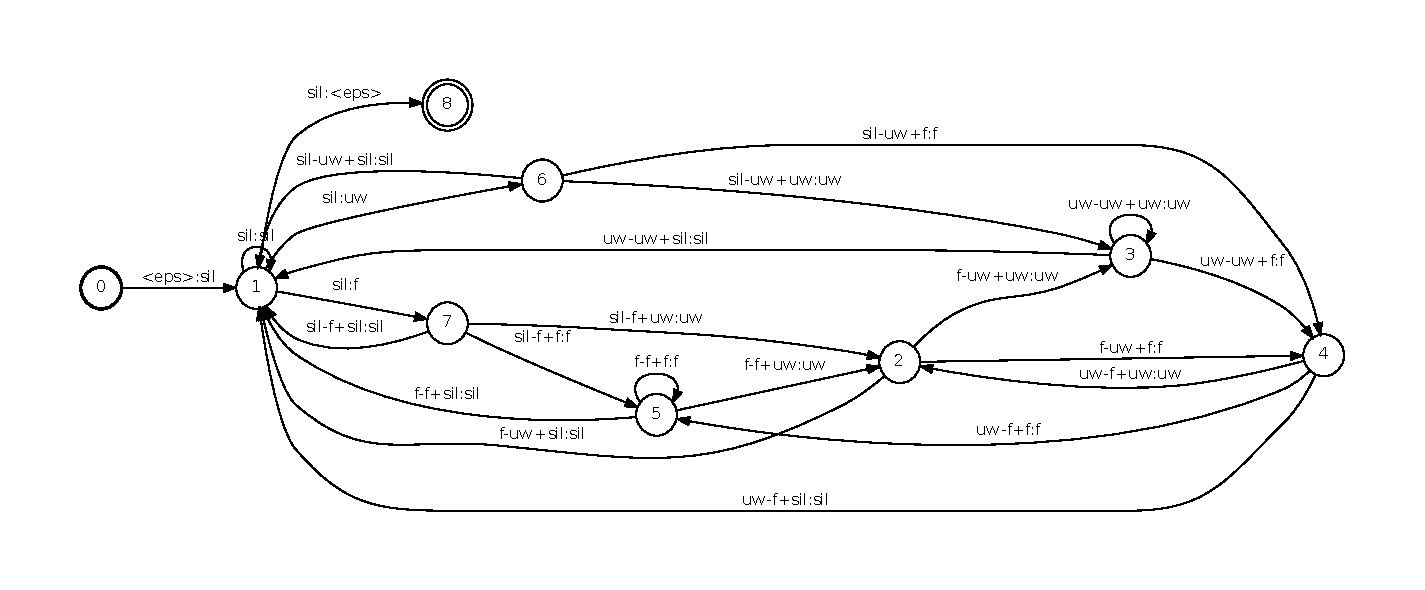
\includegraphics[width=\textwidth]{./figures/c_no_sp_aux.pdf}
  \caption{A simple cross-word type C WFST}
  \label{c_no_sp_aux}
\end{figure}

\subsection{Silence Modeling}
\label{silmod}
There are two silence models described and advocated to use in acoustic model by Young, \textit{et al}~\cite{young2006htk}. 

\begin{itemize}
\item
  A silence model, \texttt{sil}, with the same structure as the other phonetic models, acts as a context, but is context dependent.
\item
  A short pause model, \texttt{sp}, is tied to the silence model. Short pause model is context free.
\end{itemize}

\subsubsection{Silence Modeling in Juicer}
\label{juicer_sil}

There are two different routines to apply short pause model in C WFST described by Garner \textit{et al}~\cite{garner2008silence}. The insertion of \texttt{sp} into transitions in C is illustrated in Figure~\ref{c_sp_model}.

\begin{figure}[!ht] 
  \centering
  \subfloat[Juicer's implementation]{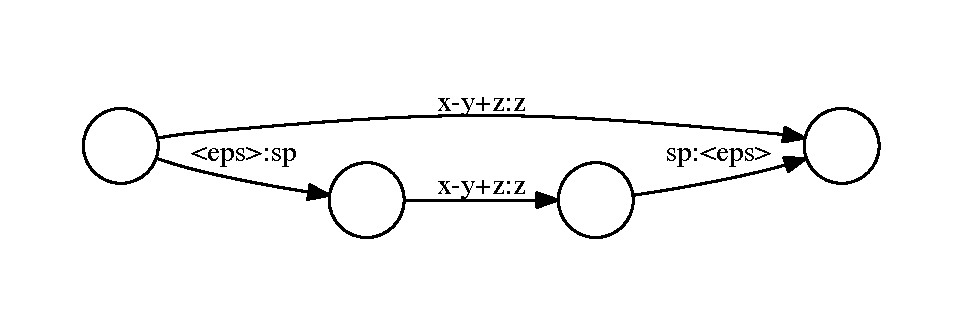
\includegraphics[width=0.6\textwidth]{./figures/c_sp1.pdf}} ~
  \subfloat[A more compact form]{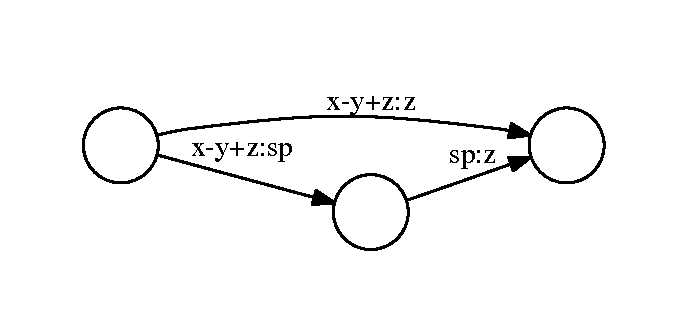
\includegraphics[width=0.4\textwidth]{./figures/c_sp2.pdf}} ~
  \caption{Insertion of \texttt{sp} into transitions in C}
  \label{c_sp_model}
\end{figure}

To accommodate silence at the lexicon level, the insertion of \texttt{sp} into transitions in L is also needed. Figure~\ref{l_sil_sp} shows the three pronounciations of a single word \texttt{NO}.

\begin{figure}[H]
  \centering
  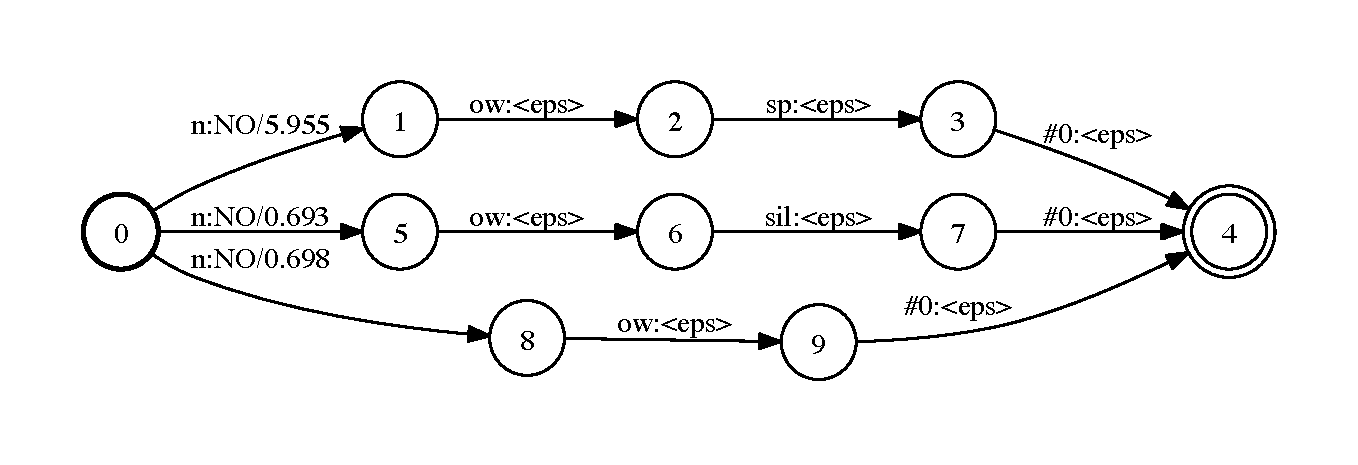
\includegraphics[width=0.8\textwidth]{./figures/l_sil_sp.pdf}
  \caption{An example of L WFST with silence phones}
  \label{l_sil_sp}
\end{figure}

\subsubsection{Silence Modeling in Transducersaurus}
\label{josef_sil}
In Transducersaurus' implementation, a silence transducer T is introduced. Thus the traditional C$\circ{}$L$\circ{}$G composition is modified to C$\circ{}$L$\circ{}$G$\circ{}$T. With this approach, silences are treated as just like other words, as described in~\cite{allauzen2004generalized}. Figure~\ref{silcls} shows the basic representation of a silence transducer T. To allow more complex silence modeling, class-based approach can be applied in transducer T. But currently only the silence transducer in Figure~\ref{silcls} is implemented.

\begin{figure}[H]
  \centering
  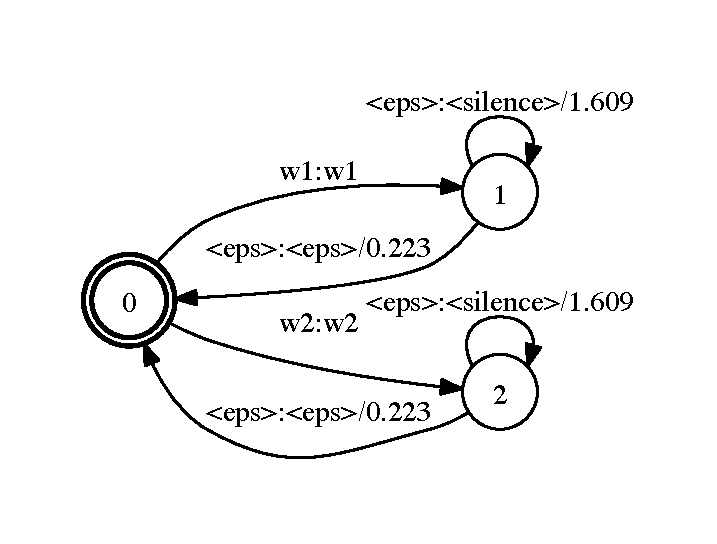
\includegraphics[width=0.5\textwidth]{./figures/silcls.pdf}
  \caption{A simple silence transducer T}
  \label{silcls}
\end{figure}

\subsection{Auxiliary Symbols}
\label{cdaux}
If the auxiliary labels are left in L$\circ$G, then C WFST must add some auxiliary transitions to match those in L$\circ$G. The easiest way to implement is to add auxiliary loops on all states of C WFST, as illustrated in Figure~\ref{c_aux}. 

\begin{figure}[H]
  \centering
  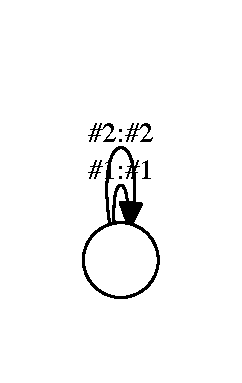
\includegraphics[width=0.2\textwidth]{./figures/c_aux.pdf}
  \caption{Auxiliary loops on states of C WFST}
  \label{c_aux}
\end{figure}

\section{Conclusion}
\label{sec:conclusion}




\bibliography{ref}

\newpage

\end{document}

